\documentclass{oblivoir}
\usepackage{amsmath,amssymb,amsthm,kotex,paralist,kswrapfig,tabu}

\usepackage[skipabove=10pt,skipbelow=10pt,innertopmargin=10pt]{mdframed}

\usepackage{tabto,pifont}
\TabPositions{0.2\textwidth,0.4\textwidth,0.6\textwidth,0.8\textwidth}
\newcommand\tabb[5]{\par\bigskip\noindent
\ding{172}\:{\ensuremath{#1}}
\tab\ding{173}\:\:{\ensuremath{#2}}
\tab\ding{174}\:\:{\ensuremath{#3}}
\tab\ding{175}\:\:{\ensuremath{#4}}
\tab\ding{176}\:\:{\ensuremath{#5}}}

\usepackage{enumitem}
\setlist[enumerate]{label=(\arabic*)}

\newcounter{num}
\newcommand{\defi}[1]
{\noindent\refstepcounter{num}\textbf{정의 \arabic{num}) #1}\par\noindent}
\newcommand{\theo}[1]
{\noindent\refstepcounter{num}\textbf{정리 \arabic{num}) #1}\par\noindent}
\newcommand{\exam}[1]
{\bigskip\bigskip\noindent\refstepcounter{num}\textbf{예시 \arabic{num}) #1}\par\noindent}
\newcommand{\prob}[1]
{\bigskip\bigskip\noindent\refstepcounter{num}\textbf{문제 \arabic{num}) #1}\par\noindent}
\newcommand{\proo}
{\bigskip\textsf{증명)}\par}

\newcommand{\procedure}[1]{\begin{mdframed}\vspace{#1\textwidth}\end{mdframed}}
\newcommand{\ans}{
{\par\raggedleft\textbf{답 : (\qquad\qquad\qquad\qquad\qquad\qquad)}\par}\bigskip\bigskip}
\newcommand\an[1]{\par\bigskip\noindent\textbf{문제 #1)}\\}

\newcommand{\pb}[1]%\Phantom + fBox
{\fbox{\phantom{\ensuremath{#1}}}}

\newcommand\ba{\,|\,}

\let\oldsection\section
\renewcommand\section{\clearpage\oldsection}

\newenvironment{talign}
 {\let\displaystyle\textstyle\align}
 {\endalign}
\newenvironment{talign*}
 {\let\displaystyle\textstyle\csname align*\endcsname}
 {\endalign}

\let\emph\textsf
%%%%
\begin{document}

\title{민형 : 04 특이적분, 도함수의 활용}
\author{}
\date{\today}
\maketitle
\tableofcontents
\newpage

%%
\section{특이적분(Improper Integral)}

%
\exam{}
다음은 \(y=\frac1{x^2}\)의 그래프이다.
이때 \(x=1\), \(y=\frac1{x^2}\), \(x\)축으로 둘러싸인 영역의 넓이를 구하여라.
\begin{figure}[h!]
\centering
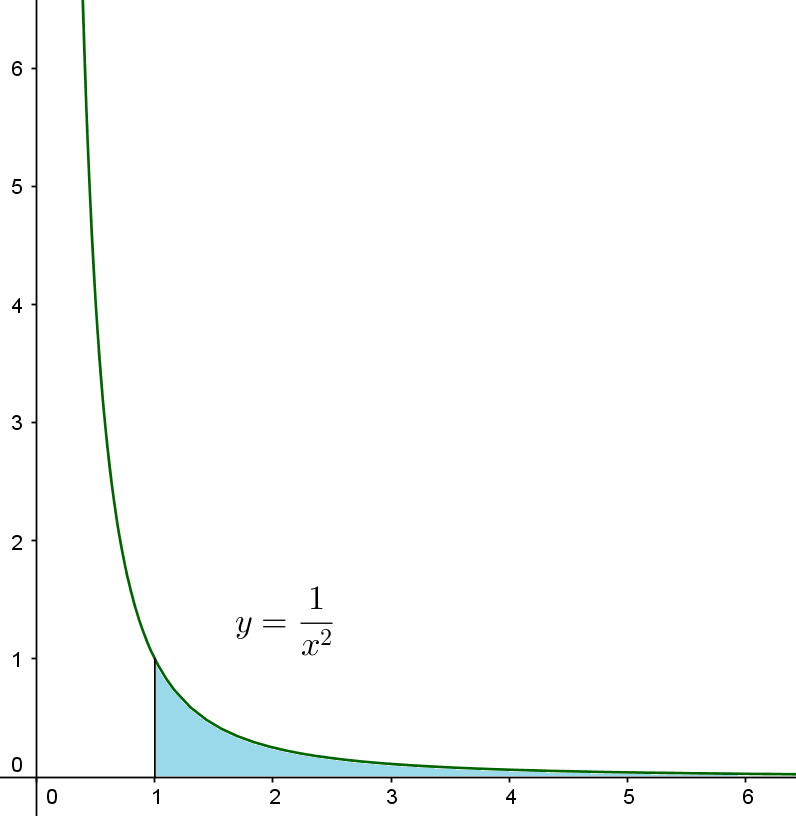
\includegraphics[width=0.6\textwidth]{frac1x^2}
\end{figure}
\procedure{0.5}
{\par\raggedleft\textbf{답 : \(1\)}\par}

\clearpage
%
\exam{}
다음은 \(y=\frac1{\sqrt x}\)의 그래프이다.
이때 \(x=1\), \(y=\frac1{\sqrt x}\), \(x\)축, \(y\)축으로 둘러싸인 영역의 넓이를 구하여라.
\begin{figure}[h!]
\centering
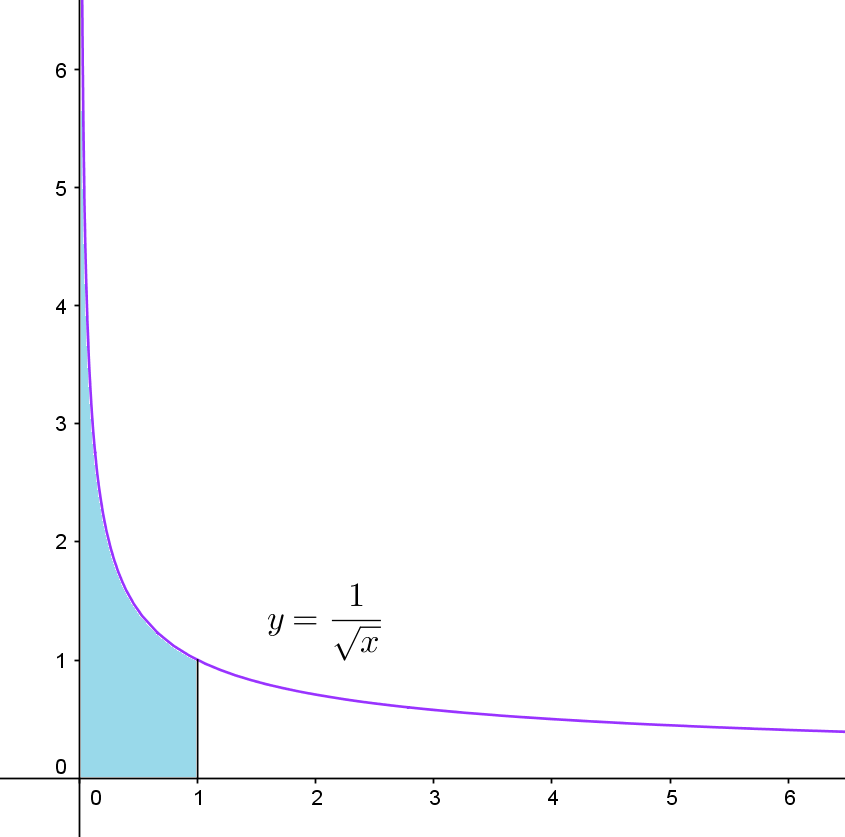
\includegraphics[width=0.6\textwidth]{frac1sqrtx}
\end{figure}
\procedure{0.7}
{\par\raggedleft\textbf{답 : \(2\)}\par}

\clearpage
%
\exam{}
다음은 \(y=\frac1{x}\)의 그래프이다.
이때 \(x=1\), \(y=\frac1{x}\), \(x\)축으로 둘러싸인 영역의 넓이를 구하여라.
\begin{figure}[h!]
\centering
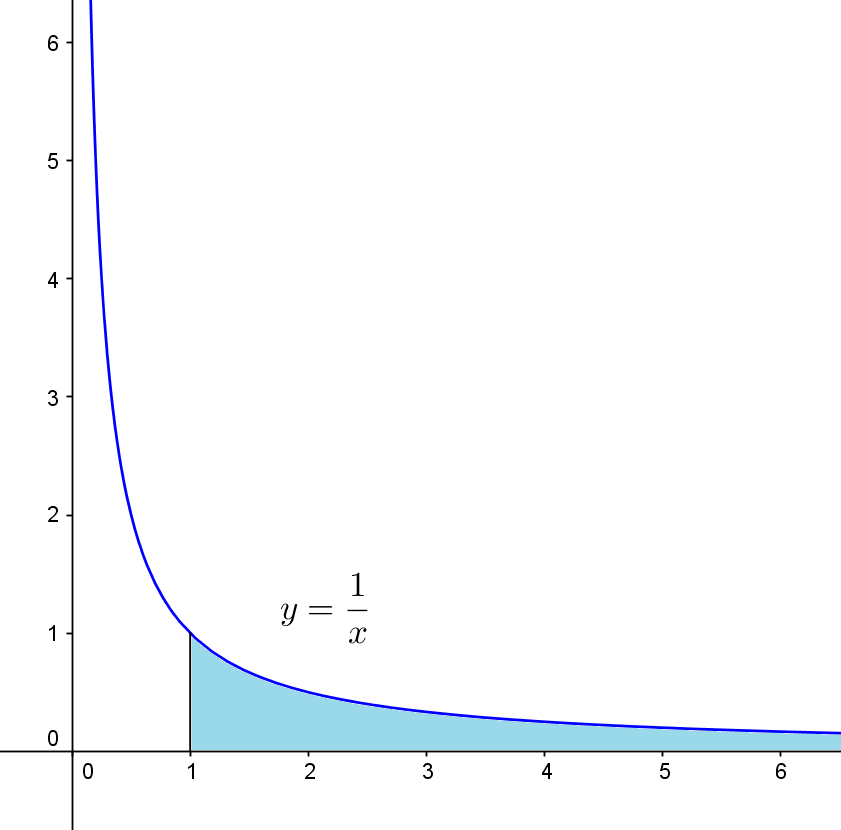
\includegraphics[width=0.6\textwidth]{frac1x}
\end{figure}
\procedure{0.7}
{\par\raggedleft\textbf{답 : \phantom{구할 수 없다(양의 무한대로 발산한다)}}\par}

\clearpage
%
\exam{}
\begin{center}
다음 급수의 수렴, 발산을 조사하여라.
\[1+\frac12+\frac13+\frac14+\cdots\]
\end{center}
\procedure{0.7}
{\par\raggedleft\textbf{답 : \phantom{양의 무한대로 발산한다}}\par}

%%
\section{접선의 방정식}

\begin{mdframed}
점 \((x_1,y_1)\)을 지나고 기울기가 \(m\)인 직선의 방정식은
\[y=m(x-x_1)+y_1\]
이다.
\end{mdframed}

\begin{mdframed}
%
\theo{}\label{formula}
함수 \(y=f(x)\)가 \(x=a\)에서 미분가능할 때, 곡선 \(y=f(x)\) 위의 점 \((a,f(a))\)에서의 접선의 방정식은
\[y=f'(a)(x-a)+f(a)\]
이다.
\end{mdframed}

%
\exam{}
원점에서 곡선 \(y=e^x\)에 그은 접선의 방정식을 구하여라.
\begin{mdframed}
\kswrapfig[Pos=r,Width=4cm]{e^x}{
\(f(x)=e^x\)으로 놓으면 \(f'(x)=e^x\)이다.
이때 접점의 좌표를 \((a,e^a)\)이라고 하면 접선의 기울기는 \(f'(a)=e^a\)이므로 구하는 접선의 방정식은
\[
y-e^a=e^a(x-a),\qquad y=e^ax-e^a(a-1)
\]
그런데 이 접선이 원점을 지나므로\\
\(0=-e^a(a-1)\) 에서 \(a=1\)이다.
따라서 구하는 접선의 방정식은 \(y=ex\)이다.
}
\end{mdframed}
{\par\raggedleft\textbf{답 : \(y=ex\)}\par}

%%
\section{함수의 증가 · 감소}

\begin{mdframed}
%
\defi{}
함수 \(y=f(x)\)가 어떤 구간에 속하는 임의의 두 수 \(x_1\), \(x_2\)에 대하여
\begin{enumerate}
\item
\(x_1<x_2\)일 때, \(f(x_1)<f(x_2)\)이면 함수 \(f(x)\)는 그 구간에서 \emph{증가}한다고 한다.
\item
\(x_1<x_2\)일 때, \(f(x_1)>f(x_2)\)이면 함수 \(f(x)\)는 그 구간에서 \emph{감소}한다고 한다.
\end{enumerate}
\end{mdframed}

\begin{mdframed}
%
\theo{}
함수 \(y=f(x)\)가 어떤 구간에서 미분가능하고 그 구간에서
\begin{enumerate}
\item
\(f'(x)>0\)이면 \(f(x)\)는 그 구간에서 증가한다.
\item
\(f'(x)<0\)이면 \(f(x)\)는 그 구간에서 감소한다.
\end{enumerate}
\end{mdframed}

%
\exam{}
위 정리의 역인
\begin{center}
\(f(x)\)가 증가함수이면 \(f'(x)>0\)이다.
\end{center}
은 성립하지 않는다.
예를 들어 함수 \(y=x^3\)은 구간 \((-1,1)\)에서 미분가능한 함수이고 증가함수이지만, 항상 \(f'(x)>0\)인 것은 아니다.
\(f'(0)=0\)이기 때문이다.

대신 다음 정리는 성립한다.

\begin{mdframed}
%
\theo{}
함수 \(y=f(x)\)가 어떤 구간에서 미분가능하고 그 구간에서
\begin{enumerate}
\item
\(f(x)\)가 증가함수이면 \(f'(x)\ge0\)이다.
\item
\(f(x)\)가 감소함수이면 \(f'(x)\le0\)이다.
\end{enumerate}
\end{mdframed}

%%
\section{함수의 극대 · 극소}
\begin{mdframed}
%
\theo{극대 / 극소 판정법 1}
함수 \(f(x)\)가
\begin{enumerate}
\item
\(x=a\)의 좌우에서 \(f(x)\)가 증가상태에서 감소상태로 바뀌면 \(f(x)\)는 \(x=a\)에서 극대이다.
\item
\(x=a\)의 좌우에서 \(f(x)\)가 감소상태에서 증가상태로 바뀌면 \(f(x)\)는 \(x=a\)에서 극소이다.
\end{enumerate}
\end{mdframed}

\begin{mdframed}
%
\theo{극대 / 극소 판정법 2}
미분 가능한 함수 \(f(x)\)가 \(f'(a)=0\)이고,
\begin{enumerate}
\item
\(x=a\)의 좌우에서 \(f'(x)\)의 부호가 양(+)에서 음(-)으로 바뀌면 \(f(x)\)는 \(x=a\)에서 극대이다.
\item
\(x=a\)의 좌우에서 \(f'(x)\)의 부호가 음(-)에서 양(+)으로 바뀌면 \(f(x)\)는 \(x=a\)에서 극소이다.
\end{enumerate}
\end{mdframed}

\begin{mdframed}
%
\theo{}
미분 가능한 함수 \(f(x)\)에 대해
\begin{center}
\(f(x)\)가 \(x=a\)에서 극값을 가지면 \(f'(a)=0\)이다.
\end{center}
\end{mdframed}

%
\exam{}
\begin{enumerate}
\item
하지만 위 정리의 역인
\begin{center}
\(f'(a)=0\)이면 \(f(x)\)가 \(x=a\)에서 극값을 가진다.
\end{center}
은 성립하지 않는다.
\(f(x)=x^3\)이면 \(f'(0)=0\)이지만 \(f(0)\)은 극값이 아니다.
\item
또, \(f(x)\)가 미분 가능하지 않으면 위의 정리는 의미가 없다.
\(f(x)=|x|\)이면 \(x=0\)에서 극값을 가지지만 \(f'(0)=0\)이라고 볼 수 없다.
\end{enumerate}

\clearpage
함수가 이계도함수를 가지는 경우 다음과 같이 판정할 수도 있다.
\begin{mdframed}
%
\theo{극대 / 극소 판정법 3}
함수 \(f(x)\)의 이계도함수 \(f''(x)\)가 존재하고 \(f'(a)=0\)일 때,
\begin{enumerate}
\item
\(f''(a)>0\)이면 \(f(x)\)는 \(x=a\)에서 극대이고, 극댓값은 \(f(a)\)이다.
\item
\(f''(a)<0\)이면 \(f(x)\)는 \(x=a\)에서 극소이고, 극솟값은 \(f(a)\)이다.
\end{enumerate}
\end{mdframed}

%
\exam{}
위 정리의 역인
\begin{center}
\(f(x)\)가 \(x=a\)에서 극대이면 \(f''(a)>0\)이다.
\end{center}
은 성립하지 않는다.
\(f(x)=-x^4\)이면 \(x=0\)에서 극댓값을 갖지만 \(f''(0)<0\)은 아니다.

%
\exam{}
\(f(x)=x^3-12x+1\)의 극값을 구하여라.
\begin{mdframed}
\begin{align*}
f'(x)&=3x^2-12=3(x-2)(x+2)\\
f''(x)&=6x
\end{align*}
이다.
판정법 2를 쓰기 위해 표를 그리면

\begin{tabu}{X[c]|X[c]|X[c]|X[c]|X[c]|X[c]}
\hline
\(x\) 	&\(\cdots\)		&\(-2\)	&\(\cdots\)			&\(2\)	&\(\cdots\)\\\hline
\(f'(x)\) 	&\(+\)			&\(0\)	&\(-\)				&\(0\)	&\(+\)\\\hline
\(f(x)\) 	&\(\nearrow\)	&\(17\)	&\(\searrow\)		&\(-15\)	&\(\nearrow\)
\\\hline
\end{tabu}
\noindent이므로 극댓값은 \(f(-2)=17\), 극솟값은 \(f(2)=-15\)이다.

판정법 3을 쓰면, \(f'(x)=0\)을 만족하는 \(x\)는 \(-2\)와 \(2\)이므로 극값을 가질 가능성이 있는 \(x\)값은 \(-2\)와 \(2\)이다.
이때 \(f''(-2)=-12<0\), \(f''(2)=12>0\)이므로 \(f(x)\)는 \(x=-2\)에서 극댓값 \(17\), \(x=2\)에서 극솟값 \(-15\)을 가진다.

\end{mdframed}

%%
\section{곡선의 볼록 · 오목}

\begin{mdframed}
\kswrapfig[Pos=r,Width=4cm]{concave}{
%
\defi{}
어떤 구간에서 곡선 \(y=f(x)\) 위의 임의의 두 점 \(P\), \(Q\)에 대하여 이 두 점 사이에 있는 곡선 부분이
\begin{enumerate}
\item
선분 \(PQ\)보다 아래쪽에 있으면\\ \(y=f(x)\)는 이 구간에서 \emph{아래로 볼록}하다고 한다.
\item
선분 \(PQ\)보다 위쪽에 있으면\\ \(y=f(x)\)는 이 구간에서 \emph{위로 볼록}하다고 한다.
\end{enumerate}
}
\end{mdframed}

위 그림에서
\(y=f(x)\)가 아래로 볼록이면 \(x\)가 증가할 수록 \(f(x)\)의 기울기가 증가하고,
\(y=f(x)\)가 위로 볼록이면 \(x\)가 증가할 수록 \(f(x)\)의 기울기가 감소함을 알 수 있다.
따라서

\begin{mdframed}
\theo{}
함수 \(f(x)\)가 어떤 구간에서
\begin{enumerate}
\item
\(f''(x)>0\)이면 곡선 \(y=f(x)\)는 이 구간에서 아래로 볼록이다.
\item
\(f''(x)<0\)이면 곡선 \(y=f(x)\)는 이 구간에서 위로 볼록이다.
\end{enumerate}
\end{mdframed}

\begin{mdframed}
%
\defi{}
곡선 \(y=f(x)\)에서 어떤 점 \(P(a,f(a)\)를 경계로 하여 오목·볼록성이 바뀌면 그 점을 \emph{변곡점}이라고 한다.
\end{mdframed}

\begin{mdframed}
%
\theo{}
함수 \(f(x)\)가 \(f''(a)=0\)이고 \(x=a\)의 좌우에서 \(f''(x)\)의 부호가 바뀌면 점 \((a,f(a))\)는 이 곡선 \(y=f(x)\)의 변곡점이다.
\end{mdframed}

\end{document}